\apendice{Documentación de usuario}

\section{Introducción}
En esta sección se va detallar como utilizar la aplicación. Como usuarios hay dos posibilidades. La versión ejecutable, que permite ver una serie de escenarios de prueba, y usar la aplicación directamente desde \textit{Unity}, lo que permite poder modificar las escenas, los parámetros y contar con una vista adicional para poder seguir el desarrollo de los algoritmos.

\section{Requisitos de usuarios}
Para poder ejecutar el proyecto desde \textit{Unity}, es necesario la versión 5.3.6 o superior, y un ordenador con cualquiera de los sistemas operativos principales (Linux, Windows y MacOS) que cuente con una tarjeta gráfica 3D.

Para el ejecutable los requisitos son los mismos solo que no es necesario usar \textit{Unity}.

Los requisitos mínimos oficiales para usar \textit{Unity} son:\footnote{Requisitos mínimos Unity: \url{https://unity3d.com/es/unity/system-requirements}}
\begin{itemize}
\item Sistema operativo Windows 7 SP1 o superior, MacOS X 10.8 o superior, Ubuntu 12.04 o superior.
\item Tarjeta gráfica con DX9 (modelo de shader 3.0) o DX11 con capacidades de funciones de nivel 9.3.
\item CPU compatible con el conjunto de instrucciones SSE2.
\end{itemize}

\section{Instalación}
El proceso de instalación para usar la aplicación con el editor de \textit{Unity} es la misma que vimos en la sección \ref{dinstalacion}.

Todos los archivos necesarios están en el repositorio de github, cuya dirección es: \href{https://github.com/vpe0001/Algoritmos\_de\_busqueda\_3D-Unity}{Repositorio del proyecto}\footnote{Repositorio del proyecto: \url{https://github.com/vpe0001/Algoritmos\_de\_busqueda\_3D-Unity}}

Para descargarlo, se puede usar git o descargar el archivo zip y descomprimir los ficheros. Desde \textit{Unity}, se abre el proyecto que se encuentra en la carpeta \textit{Codigo\textbackslash Algoritmos\_de\_busqueda\_3D}, o bien se crea un proyecto nuevo y se importa el paquete del directorio \textit{Exportar}, desde \textit{Assets-\textgreater Import Package}.

El ejecutable no requiere de instalación adicional. Los archivos ejecutables se encuentran en la carpeta\textit{Build}, en la que a su vez hay dos carpetas, una para la versión Linux, y otra para la versión Windows.

\section{Manual del usuario}
\subsection{Manual para \textit{Unity}}
Una vez realizada la instalación, abriremos el proyecto con \textit{Unity}. Cuando se inicie, nos encontremos en la interfaz del editor de \textit{Unity}. Desde \textit{File-\textgreater Open Scene} podemos cargar la escena que deseemos probar. Nos encontraremos una pantalla similar a la de la figura \ref{fig:dunityui}.

\begin{figure}[htpb]
    \centering
    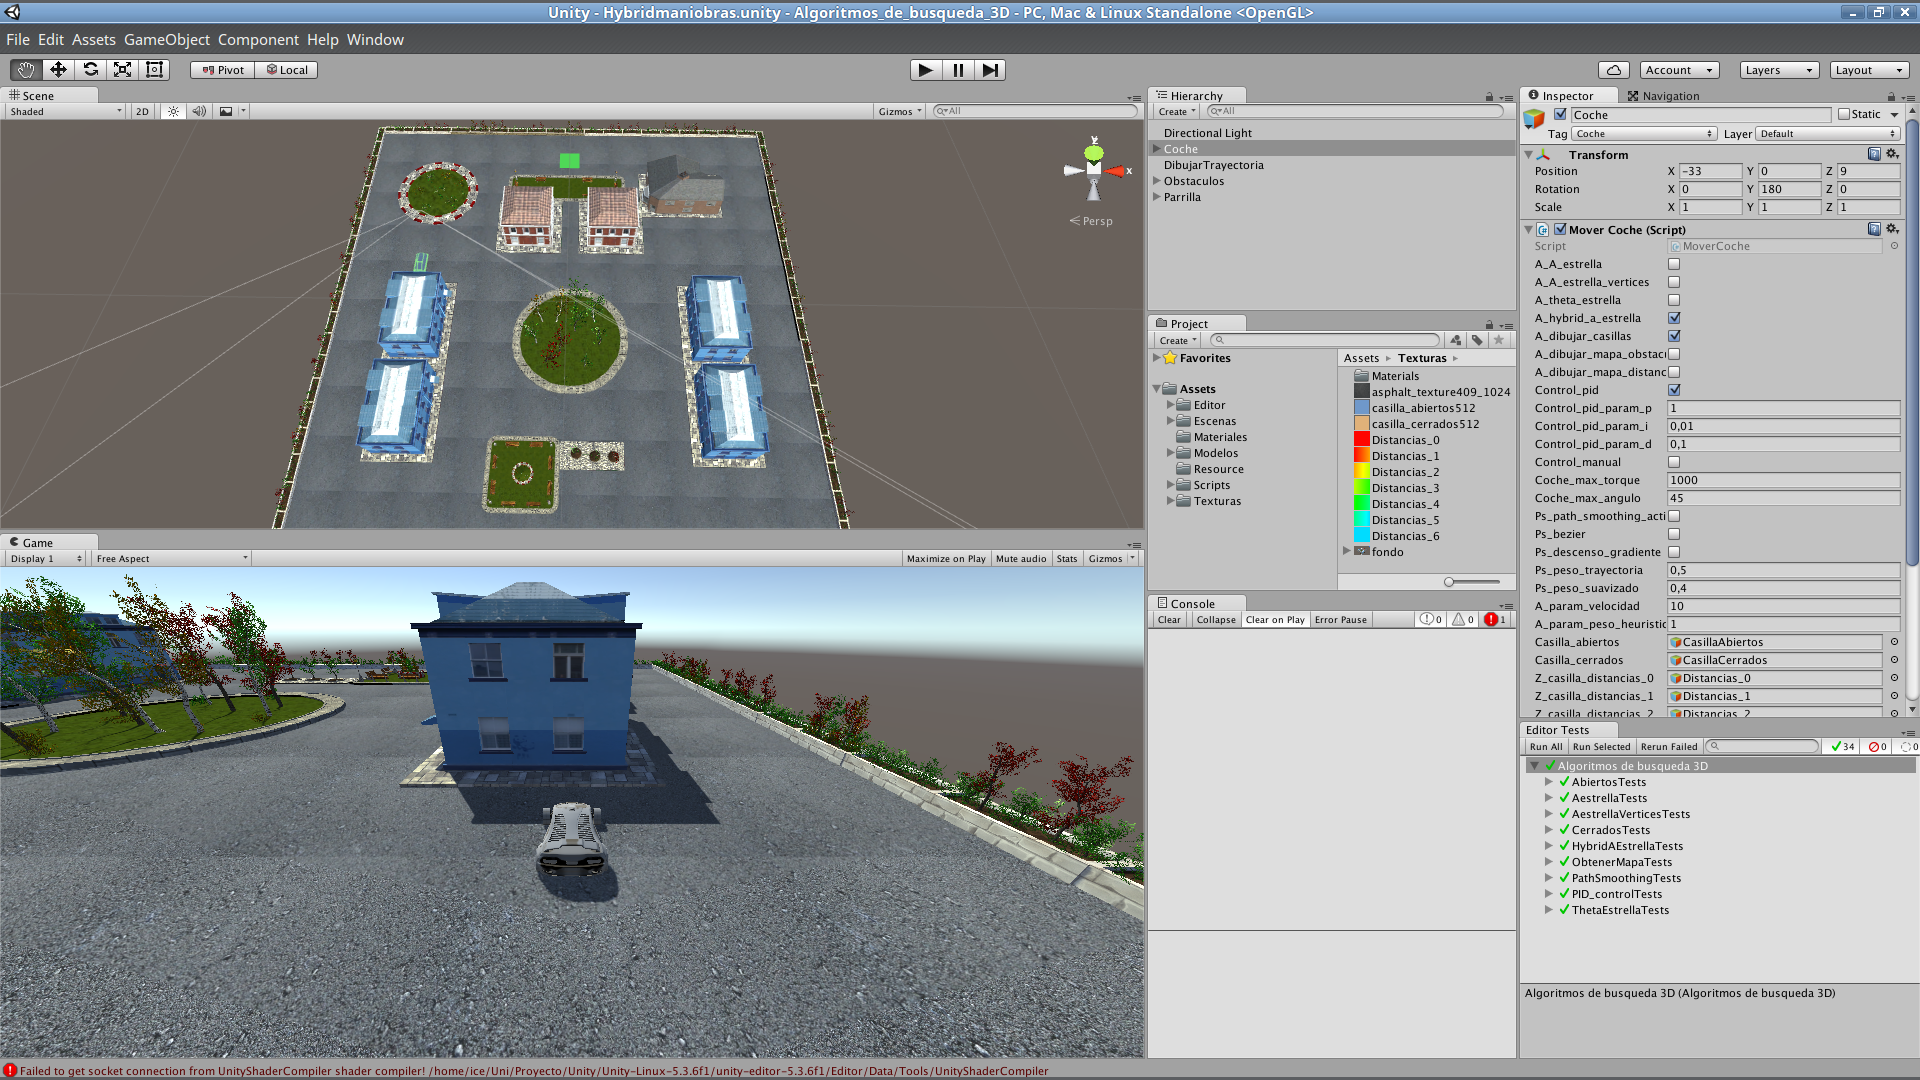
\includegraphics[width=\textwidth,height=8cm,keepaspectratio=true]{d_unityui}
    \caption[Pantalla de la interfaz de \textit{Unity}]{Pantalla de la interfaz de \textit{Unity}.}
    \label{fig:dunityui}
\end{figure}

A la izquierda, tenemos dos vistas de la escena en tres dimensiones. La de arriba corresponde al editor, y nos permite colocar la cámara en cualquier momento donde deseemos haciendo \textit{click} con el ratón. Esta vista es útil para tener un perspectiva de la escena completa, y poder observar como se desarrollan los algoritmos por ella. En la vista de abajo se encuentra la perspectiva desde el vehículo. Esta vista es útil cuando se realiza el seguimiento de la ruta, para poder observar el desplazamiento del vehículo.

Las dos columnas de la derecha corresponden a los elementos del proyecto. \textit{Hierarchy} contiene los elementos de la escena que podemos seleccionar para modificarles, mientras que \textit{Project} muestra todos los \textit{assets} del proyecto que podemos usar para crear las distintas escenas.

\textit{Inspector} mostrará los parámetros de los elementos seleccionados, y es donde vamos a modificar los distintos valores de los algoritmos. Seleccionando Coche en \textit{Hierarchy} y nos mostrará los valores que podemos configurar en el proyecto:
\begin{itemize}
\item \textbf{\textit{Transform}}: donde podemos modificar la posición (los valores de \textit{Position}) y la orientación del vehículo (el valor $y$ de \textit{Rotation}). También está disponible para el resto de los elementos como los obstáculos
\item A continuación aparecen los cuatro algoritmos disponibles para seleccionar: el A*, Theta*, A* con vértices y Hybrid A*.
\item Las opciones de \textit{dibujar mapa obstáculos} y \textit{dibujar mapa distancias} muestran respectivos mapas al inicio de la ejecución. Aunque no es recomendable realizar la ejecución completa con los mapas activados puesto que, además de perder visibilidad, el rendimiento debido al gran número de elementos en pantalla se reduce considerablemente.
\item La opción siguiente nos permite activar el \textit{PID Controller} para el movimiento autónomo del vehículo, y podemos modificar los parámetros \textit{P}, \textit{I} y \textit{D} para comprobar como afectan al movimiento.
\item Control manual nos permite, una vez activado, manejar al vehículo con las teclas del teclado.
\item Con \textit{Path Smoothing} activamos el suavizado de la ruta. Si no activamos las opciones de \textit{Descenso Gradiente} ni \textit{Curvas Bézier}, realizará la eliminación del zigzag. Si no, realizará la opción seleccionada. También es posible modificar los valores de los parámetros del \textit{Descenso gradiente} y ver las distintas rutas que genera.
\item La opción de \textit{param velocidad} se utiliza cuando no se ha seleccionado ni \textit{PID control} ni \textit{control manual}. En ese caso el vehículo no se moverá a usando las físicas, si no que se trasladará a través de la ruta hasta la meta a la velocidad que indica ese parámetro.
\item El parámetro \textit{peso heurísticas} sirve para configurar cuanta importancia tendrá la función H() en las rutas generadas en relación a la función G(). Si el valor es grande, el algoritmo búscará más en anchura, mientras que si es pequeño, intentará antes acercarse a la meta.
\end{itemize}

\subsection{Manual para el ejecutable}
La versión ejecutable es una aplicación reducida de lo que se puede hacer desde \textit{Unity}. Consiste en un menú principal donde se pueden escoger ocho escenas preconfiguradas.

Para ejecutarlo se hace doble \textit{click}, a continuación aparecen las opciones gráficas de resolución y preajustes de calidad de la imagen disponibles. Pulsando aceptar se inicia el menú de la aplicación, como se muestra en la figura \ref{fig:dmenuejecutable}\footnote{\textit{Unity} no permite el uso de acentos en los elementos de texto para la interfaz}.

\begin{figure}[htpb]
    \centering
    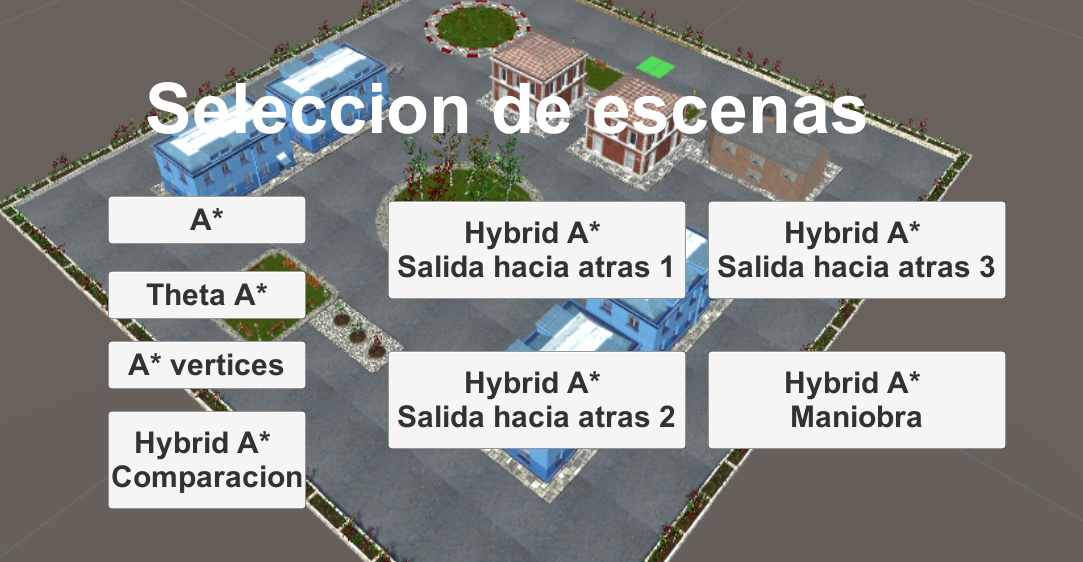
\includegraphics[width=\textwidth,height=8cm,keepaspectratio=true]{d_menuejecutable}
    \caption[Pantalla del menú del ejecutable]{Pantalla del menú del ejecutable.}
    \label{fig:dmenuejecutable}
\end{figure}

Para usarlo, hacemos \textit{click} en el botón correspondiente y se ejecutará la escena asociada. Cuando el vehículo llegue a la meta, la ejecución habrá terminado y se puede cerrar la ventana. Para cargar otra escena repetimos el proceso.

La columna de botones de la izquierda corresponden al mismo escenario, pero cada uno con un algoritmo diferente para poder compararles. Los cuatro botones restantes corresponden al \textit{Hybrid A*}, donde el vehículo realiza distintas maniobras.

